\documentclass{article}


\usepackage{arxiv}

\usepackage[utf8]{inputenc} % allow utf-8 input
\usepackage[T1]{fontenc}    % use 8-bit T1 fonts
\usepackage{hyperref}       % hyperlinks
\usepackage{url}            % simple URL typesetting
\usepackage{booktabs}       % professional-quality tables
\usepackage{amsfonts}       % blackboard math symbols
\usepackage{nicefrac}       % compact symbols for 1/2, etc.
\usepackage{microtype}      % microtypography
\usepackage{lipsum}
\usepackage{graphicx}
\usepackage{subcaption} 
%\graphicspath{ {./images} }
\usepackage[rightcaption]{sidecap}
\usepackage{wrapfig}
\usepackage{amsmath}
\usepackage{fancyvrb}
\usepackage{braket}
\usepackage{bbold}



\usepackage{listings}
\usepackage{color}

\definecolor{dkgreen}{rgb}{0,0.6,0}
\definecolor{gray}{rgb}{0.5,0.5,0.5}
\definecolor{mauve}{rgb}{0.58,0,0.82}

\lstset{frame=tb,
  language=C++,
  aboveskip=3mm,
  belowskip=3mm,
  showstringspaces=false,
  columns=flexible,
  basicstyle={\small\ttfamily},
  numbers=none,
  numberstyle=\tiny\color{gray},
  keywordstyle=\color{blue},
  commentstyle=\color{dkgreen},
  stringstyle=\color{mauve},
  breaklines=true,
  breakatwhitespace=true,
  tabsize=3
}

\title{Restricted Boltzmann machine representation for the groundstate and excited states of Kitaev Honeycomb model}


\author{
    Mohammadreza Noormandipour\thanks{\texttt{mrn31@cam.ac.uk}}\hspace{1mm}$^{,a}$ , Youran Sun\thanks{\texttt{mrn31@cam.ac.uk}}\hspace{1mm}$^{,b}$ , Babak Haghighat\thanks{\texttt{babakhaghighat@tsinghua.edu.cn}}\hspace{1mm}$^{,b}$ \\
	$^{a}$ \textit{DAMTP}, University of Cambridge, Wilberforce Road, Cambridge CB3 0WA, UK \\
	$^{b}$ \textit{Yau Mathematical Sciences Center}, Tsinghua University, Beijing, 100084, China\\
      %% David S.~Hippocampus\thanks{Use footnote for providing further
  %%  information about author (webpage, alternative
  %%    address)---\emph{not} for acknowledging funding agencies.} \\
  %% Department of Computer Science\\
  %% Cranberry-Lemon University\\
  %% Pittsburgh, PA 15213 \\
  %% \texttt{hippo@cs.cranberry-lemon.edu} \\
  %% examples of more authors
  %% \And
 %% Elias D.~Striatum \\
  %% Department of Electrical Engineering\\
  %% Mount-Sheikh University\\
  %% Santa Narimana, Levand \\
  %% \texttt{stariate@ee.mount-sheikh.edu} \\
  %% \AND
  %% Coauthor \\
  %% Affiliation \\
  %% Address \\
  %% \texttt{email} \\
  %% \And
  %% Coauthor \\
  %% Affiliation \\
  %% Address \\
  %% \texttt{email} \\
  %% \And
  %% Coauthor \\
  %% Affiliation \\
  %% Address \\
  %% \texttt{email} \\
}

\begin{document}
\maketitle

\begin{abstract}
%\lipsum[1]
In this work, the capability of restricted Boltzmann machines (RBMs) to find solutions for the Kitaev honeycomb model is investigated. The measured groundstate (GS) energy of the system is compared and shown to reside within less than $1\%$ error of the analytically derived value of the energy. Furthermore, the possibility of realizing anyons in the RBM is discussed and an algorithm is given to build these anyonic excitations and braid them as a proof of concept for performing quantum gates and doing quantum computation. Moreover, the phase transition of the system is also studied by changing the corresponding hyperparameters of the system in the RBM solution.
\end{abstract}


% keywords can be removed
\keywords{Restricted Boltzmann Machine (RBM) \and Honeycomb Lattice Model \and Topological Phases of Matter \and Anyons \and Quantum Computing}


\section{Introduction}
%\lipsum[2]
%\lipsum[3]
Honeycomb model is a 2-dimensional lattice spin system (see Fig.\hspace{0.2mm}\ref{fig:fig0}) which was first introduced by Kitaev in 2006 \cite{kita} and is famous because of the topological quantum order due to a degenerate gapped groundstate which is persistent to local and finite-sized perturbations. The system also supports both abelian and non-abelian topological phases as demonstrated in the original proposal \cite{kita}. There is a wide range of applications for this model, from fault-tolerant quantum computation \cite{kita2} to analytical study of strongly correlated systems \cite{str-cor} and quantum spin liquids \cite{spi-liq}. The honeycomb lattice is not a Bravias lattice in its original structure, but it can be considered as a triangular Bravias lattice with a two-spin basis. The direct Bravias lattice and the primitive cells are illustrated in Fig.\hspace{0.2mm}\ref{fig:fig0}a with the dashed lines. Each primitive cell has a pair of odd and even indexed spins. Just for the sake of simplicity we will denote each cell with the even indexed (empty circles) spins of the system. The primitive vectors of the lattice, $\textbf{a}_1$ and $\textbf{a}_2$ are also shown in Fig.\hspace{0.2mm}\ref{fig:fig0}a (see also Equ.\hspace{0.2mm}\ref{eq:0}). The entire lattice can be tiled and covered with primitive cells using translations composed of different linear combinations of primitive vectors. 

\begin{equation}\label{eq:0}
    \textbf{a}_1 = \sqrt{3} a \textbf{e}_x \hspace{1cm} \& \hspace{1cm}
    \textbf{a}_2 = \frac{\sqrt{3}}{2} a (\textbf{e}_x, \sqrt{3}\textbf{e}_y)
\end{equation}

Where 'a' is the lattice constant. The reciprocal lattice for the triangle lattice can be obtained by solving Equ.\hspace{0.2mm}\ref{eq:01} for basis vectors of the reciprocal lattice, $\textbf{b}_1$ and $\textbf{b}_2$.

\begin{equation}\label{eq:01}
    \textbf{a}_i.\textbf{b}_j = 2\pi\delta_{ij}
\end{equation}

The solution is as below:

\begin{equation}\label{eq:02}
    \textbf{b}_1 = \frac{2\pi}{\sqrt{3}a} (\textbf{e}_x-\frac{1}{\sqrt{3}}\textbf{e}_y) \hspace{1cm} \& \hspace{1cm}
    \textbf{b}_2 = \frac{4\pi}{3a} \textbf{e}_y
\end{equation}

The reciprocal lattice is depicted in Fig.\hspace{0.2mm}\ref{fig:fig0}b. The shaded region in the figure is the first Brillouin zone.

The Hamiltonian of the Kitaev model is a nearest-neighbor interaction of Pauli matrices on a honeycomb lattice as written in Equ.\hspace{0.2mm}\ref{eq:1}, where $r \& r^{'}$ are indices for the nearest neighbour spins. The physics of the system is symmetric under permutation of coupling strengths $J_{\alpha}$ with $\alpha = x, y, z$ and due to an-isotropic interaction the model is a fraustrated spin system, because a spin cannot satisfy conflicting
 demands of orientation from its three neighboring sites \cite{kita}.

\begin{equation}\label{eq:1}
    H = - \sum_{\alpha} J_{\alpha} \sum_{\alpha-bonds} \sigma^{\alpha}_{r}\sigma^{\alpha}_{r^{'}}
\end{equation}

\begin{figure}[h!]
%     \begin{subfigure}
     \centering
%     \includegraphics[width=0.8\textwidth]{./images/Final_A_2}
%     \caption{1a}
%     \label{fig:fig0a}
%     \end{subfigure}%
% 	\begin{subfigure}
%     \centering
%     \includegraphics[width=0.8\textwidth]{./images/Final_A}
%     \caption{1b}
%     \label{fig:fig0b}
%     \end{subfigure}%
    \subfloat[1a]{\includegraphics[width=0.7\textwidth]{./images/Final_A_2}}\\
    \subfloat[1b]{\includegraphics[width=0.8\textwidth]{./images/br_zone_v2}}
    \caption{plots of....}
    \label{fig:fig0}
\end{figure}

\begin{figure}[h!]
	\centering
	\includegraphics[width=0.8\textwidth]{./images/diag_1.png}
	\caption{\label{tab:r_space} Kitaev Honeycomb lattice model on a torus: The generators of the lattice in position space are named
	$\textbf{e}_{1}$ and  $\textbf{e}_{2}$, as shown in the image above. Hence, the lattice points are $\textbf{L} = n_{1}\textbf{e}_{1} + 
	n_{2}\textbf{e}_{2}$ with $n_{1}, n_{2} \in \mathbb{Z}$ and the above lattice is drawn for $N_{1} = N_{2} = 4 $ with toric boundary conditions.} 
	\label{fig:fig1}
\end{figure}


% \section{The model}

% \noindent $\bullet$\hspace{4mm} The model can be mapped to a model of p-wave BCS theory with site-dependent chemical potential for spinless fermions on a square lattice \cite{2}.

% Insert the lattice pictures in here.


\section{Solution of the Model}

In this section an exact solution of the system is provided and an explicit form of the groundstate energy is achieved. First of all, we Fermionize the Hamiltonian by performing a one dimensional Jordan-Wigner transformation \cite{nus-9-10} defined in Equ.\hspace{0.2mm}\ref{eq:2}. A deformation of the hexagonal lattice to a brick-wall lattice (see Fig.\hspace{0.2mm}\ref{fig:fig-}) clarifies the mechanism of the Jordan-Wigner transformation and why it is one dimensional. In the brick-wall lattice, each lattice site $r$ is denoted by the coordinates $(i,j)$.

\begin{equation}\label{eq:2}
	\begin{aligned}
		\sigma^{+}_{i,j} &= 2[\prod_{j'<j}\prod_{i'}\sigma^{z}_{i',j'}][\prod_{i'<i}\sigma^z_{i',j}] a^{\dagger}_{i,j}\\
		\sigma^{-}_{i,j} &= 2[\prod_{j'<j}\prod_{i'}\sigma^{z}_{i',j'}][\prod_{i'<i}\sigma^z_{i',j}] a_{i,j}\\
		\sigma^{z}_{i,j} &= 2a^{\dagger}_{i,j}a_{i,j} - 1
	\end{aligned}
\end{equation}\\

\noindent This transformation maps the Hilbert space of spins to the Hilbert space of spinless complex fermions \cite{schmull}. Using the fact that $ \sigma^{\pm} = \sigma^{x}\pm i\sigma^{y} $ one can expand the Hamiltonian in Equ.\hspace{0.2mm}\ref{eq:1} into three terms and re-write them as below.


\begin{equation}\label{eq:3}
	\begin{aligned}
		\sigma^{x}_{i,j}\sigma^{x}_{i+1,j} &= \prod_{i'<i}\sigma^z_{i',j} (a^{\dagger}_{i,j} + a_{i,j}) \prod_{i'<i+1}\sigma^z_{i',j} (a^{\dagger}_{i+1,j} + a_{i+1,j})\\
		&= (a^{\dagger}_{i,j} + a_{i,j}) \sigma^z_{i,j} (a^{\dagger}_{i+1,j} + a_{i+1,j})\\
		&= -(a^{\dagger}_{i,j} - a_{i,j}) (a^{\dagger}_{i+1,j} + a_{i+1,j})\\
		\sigma^{y}_{i,j}\sigma^{y}_{i+1,j} &= -\prod_{i'<i-1}\sigma^z_{i',j} (a^{\dagger}_{i-1,j} - a_{i-1,j}) \prod_{i'<i}\sigma^z_{i',j} (a^{\dagger}_{i,j} - a_{i,j})\\
		&= -(a^{\dagger}_{i-1,j} - a_{i-1,j}) \sigma^z_{i-1,j} (a^{\dagger}_{i,j} - a_{i,j})\\
		&= (a^{\dagger}_{i-1,j} + a_{i-1,j}) (a^{\dagger}_{i,j} - a_{i,j})\\
		\sigma^{z}_{i,j}\sigma^{z}_{i,j+1} &=  (2a^{\dagger}_{i,j}a_{i,j} - 1) (2a^{\dagger}_{i,j+1}a_{i,j+1} - 1)\\
	\end{aligned}
\end{equation}\\

\noindent Therefore, the Hamiltonian transforms to the one in Equ.\hspace{0.2mm}\ref{eq:4}. 

\begin{equation}\label{eq:4}
	\begin{aligned}
		H= &+J_x \sum_{x-links} (a^{\dagger}_{i,j} - a_{i,j}) (a^{\dagger}_{i+1,j} + a_{i+1,j})\\
		&-J_y \sum_{y-links} (a^{\dagger}_{i-1,j} + a_{i-1,j}) (a^{\dagger}_{i,j} - a_{i,j})\\
		&-J_z \sum_{z-links} (2a^{\dagger}_{i,j}a_{i,j} - 1) (2a^{\dagger}_{i,j+1}a_{i,j+1} - 1)\\
	\end{aligned}
\end{equation}\\

\noindent The $J_x$ and $J_y$ terms are quadratic interactions in spinless fermions and are easy to solve, however, the $J_z$ term is a product of number density operators and can be further simplified by introducing the Majorana operators in Equ.\hspace{0.2mm}\ref{eq:5} \cite{schmull}. As we will see, this simplification can be done due to the presence of the conserved quantity called plaquette operator $B_p$ \cite{schmull}. 

\begin{equation}\label{eq:5}
	\begin{aligned}
		c_{i,j} &= i(a^{\dagger}_{i,j} - a_{i,j}) \hspace{2mm},\hspace{2mm} d_{i,j} = a^{\dagger}_{i,j} + a_{i,j} \hspace{2mm},\hspace{2mm} for \hspace{2mm} i+j=even \equiv \circ\\
		c_{i,j} &= a^{\dagger}_{i,j} + a_{i,j} \hspace{2mm},\hspace{2mm} d_{i,j} = i(a^{\dagger}_{i,j} - a_{i,j}) \hspace{2mm},\hspace{2mm} for \hspace{2mm} i+j=odd \equiv \color{black}\bullet\\
	\end{aligned}
\end{equation}\\

\noindent These operators have the following commutation relations:

\begin{equation}\label{eq:6}
	\begin{aligned}
		&c^2_{i,j} = d^2_{i,j} = 1\\
		&\{ c_{i,j},c_{i',j'} \} = \{ d_{i,j},d_{i',j'} \} = 2\delta_{ii'} \delta_{jj'}\\
		&\{ c_{i,j},d_{i',j'} \} = 0\\
	\end{aligned}
\end{equation}\\

\noindent Then, the $J_z$ term can be rewritten using the Majorana operators: 

\begin{equation}\label{eq:7}
	\begin{aligned}
		\sigma^{z}_{i,j}\sigma^{z}_{i,j+1} &=  (2a^{\dagger}_{i,j}a_{i,j} - 1) (2a^{\dagger}_{i,j+1}a_{i,j+1} - 1)\\
		&= i(id_{i,j+1}d_{i,j})c_{i,j+1}c_{i,j} 
	\end{aligned}
\end{equation}\\

\noindent Finally, using the circle indices for the odd and even lattice sites as defined in Equ.\hspace{0.2mm}\ref{eq:5} the Hamiltonian transforms to the expression in Equ.\hspace{0.2mm}\ref{eq:8}.

\begin{equation}\label{eq:8}
	\begin{aligned}
		H= &-iJ_x \sum_{x-links} c_{\circ}c_{\color{black}\bullet}\\
		&+iJ_y \sum_{y-links} c_{\color{black}\bullet}c_{\circ}\\
		&-iJ_z \sum_{z-links} (id_{\color{black}\bullet}d_{\circ})c_{\color{black}\bullet}c_{\circ}\\ 
	\end{aligned}
\end{equation}\\

\noindent If we write the Hamiltonian as a sum over unit cells we have:

\begin{equation}\label{eq:9}
	\begin{aligned}
		H= i\sum_{\textbf{r}}[J_x c_{\color{black}\bullet,\textbf{r}}c_{\circ,\textbf{r}+\textbf{r}_1} + J_y c_{\color{black}\bullet,\textbf{r}}c_{\circ,\textbf{r}+\textbf{r}_2} - J_z (id_{\color{black}\bullet,\textbf{r}}d_{\circ,\textbf{r}})c_{\color{black}\bullet,\textbf{r}}c_{\circ,\textbf{r}}]\\ 
	\end{aligned}
\end{equation}\\

\noindent where \textbf{r} is the position vector of z-bonds or unit cells (see Fig.\hspace{0.2mm}\ref{fig:fig6.6}). It makes no difference in physics if we set \textbf{r} on every point along the z-bond, whether it is on even site or odd site or some where in the middle of them, that's a matter of translation! 
What which will be important in what follows, is that now since we have grouped a pair of even and odd sites as an unit cell, to evaluate the summation over the unit cells, it is sufficient to just run over the even or odd sites.\\
Furthermore, the $\alpha_\textbf{r} = (id_{\color{black}\bullet,\textbf{r}}d_{\circ,\textbf{r}})$ operators are defined on each z-bond of the lattice (labled by \textbf{r}) and they commute with Hamiltonian and are good quantum numbers.
Moreover, it can easily be shown that each plaquette operator shall be written as:

\begin{equation}\label{eq:10}
	\begin{aligned}
		B_p = \sigma^y_1\sigma^z_2\sigma^x_3\sigma^y_4\sigma^z_5\sigma^x_6 = \alpha_{61}\alpha_{43}\\
	\end{aligned}
\end{equation}

\noindent On the other hand, from the Lieb's theorem \cite{Lieb} we know that the groundstate manifold is obtained by setting $B_p = 1, \forall p$. 
Thus the uniform choice of $\alpha_\textbf{r}=1, \forall \textbf{r}$ corresponds to a vortex-free sector, nevertheless all configurations leading to the same sector are equivalent.\\

\noindent We also intoduce a Dirac fermion on each z-link using the Majorana operators:

\begin{equation}\label{eq:11}
	\begin{aligned}
		d_\textbf{r} &= \frac{1}{2} (c_{\color{black}\bullet,\textbf{r}} - ic_{\circ,\textbf{r}})\\
		d^\dagger_\textbf{r} &= \frac{1}{2} (c_{\color{black}\bullet,\textbf{r}} + ic_{\circ,\textbf{r}})
	\end{aligned}
\end{equation}\\

\noindent Using the inverse transformation we can rewrite the Hamiltonian:

\begin{equation}\label{eq:12}
	\begin{aligned}
		H= &\sum_{\textbf{r}}[J_x (d^\dagger_{\textbf{r}} + d_{\textbf{r}})(d^\dagger_{\textbf{r}+\textbf{r}_1} - d_{\textbf{r}+\textbf{r}_1}) \\
		&+J_y (d^\dagger_{\textbf{r}} + d_{\textbf{r}})(d^\dagger_{\textbf{r}+\textbf{r}_2} - d_{\textbf{r}+\textbf{r}_2}) \\
		&+J_z \alpha_\textbf{r}(2d^\dagger_{\textbf{r}}d_{\textbf{r}}-1)]\\ 
	\end{aligned}
\end{equation}\\

\noindent The Hamiltonian is translational invariant and can be transformed to momentum space in order to be diagonalized. We define the Fourier transformation for the Dirac fermion as:

\begin{equation}\label{eq:13}
	\begin{aligned}
		d_{\textbf{r}} &= \frac{1}{\sqrt{N}}\sum_\textbf{k} e^{+i\textbf{k}.\textbf{r}}d_{\textbf{k}} \\
		d^\dagger_{\textbf{r}} &= \frac{1}{\sqrt{N}}\sum_\textbf{k} e^{-i\textbf{k}.\textbf{r}}d^\dagger_{\textbf{k}} \\
	\end{aligned}
\end{equation}\\

\noindent Setting $\textbf{k} \rightarrow \textbf{-k}$ in $d^\dagger_\textbf{r}$ simplifies the calculations. Then we have:

\begin{equation}\label{eq:14}
	\begin{aligned}
		\textbf{X}: \hspace{2mm} &J_x\frac{1}{N}\sum_\textbf{r}\sum_{\textbf{k},\textbf{k}'}e^{+i\textbf{k}.\textbf{r}}e^{+i\textbf{k}'.(\textbf{r}+\textbf{r}_1)}(d^\dagger_{-\textbf{k}} + d_{\textbf{k}})(d^\dagger_{-\textbf{k}'} - d_{\textbf{k}'})\\
		&= J_x\sum_{\textbf{k}} [-2cos(k_1)d^\dagger_{\textbf{k}}d_{\textbf{k}} + isin(k_1)(d^\dagger_{\textbf{k}}d^\dagger_{-\textbf{k}}-h.c.)]\\
		\textbf{Y}: \hspace{2mm} &J_y\frac{1}{N}\sum_\textbf{r}\sum_{\textbf{k},\textbf{k}'}e^{+i\textbf{k}.\textbf{r}}e^{+i\textbf{k}'.(\textbf{r}+\textbf{r}_2)}(d^\dagger_{-\textbf{k}} + d_{\textbf{k}})(d^\dagger_{-\textbf{k}'} - d_{\textbf{k}'})\\
		&= J_y\sum_{\textbf{k}} [-2cos(k_2)d^\dagger_{\textbf{k}}d_{\textbf{k}} + isin(k_2)(d^\dagger_{\textbf{k}}d^\dagger_{-\textbf{k}}-h.c.)]\\
		\textbf{Z}: \hspace{2mm} &J_z\frac{1}{N}\sum_\textbf{r}\sum_{\textbf{k},\textbf{k}'}e^{+i\textbf{k}.\textbf{r}}e^{+i\textbf{k}'.\textbf{r}}(2d^\dagger_{-\textbf{k}}d^\dagger_{\textbf{k}'}-1)\\
		&= J_z\sum_{\textbf{k}} 2d^\dagger_{\textbf{k}}d_{\textbf{k}}-J_zN.\\
	\end{aligned}
\end{equation}\\

\noindent For the above equation we used the orthogonality relation in Fourier transformation:

\begin{equation}\label{eq:15}
	\begin{aligned}
		\sum_\textbf{r} e^{i(\textbf{k}+\textbf{k}').\textbf{r}} = N\delta(\textbf{k} + \textbf{k}')
	\end{aligned}
\end{equation}\\

Using all previous transformations we obtain a Hamiltonian which is quadratic in the Dirac fermions living on each of the unit cells along the z-links:

\begin{equation}\label{eq:16}
	\begin{aligned}
		H = \sum_\textbf{k}[\epsilon_\textbf{k}d^\dagger_{\textbf{k}}&d_{\textbf{k}} + \frac{1}{2}(i\Delta_\textbf{k}d^\dagger_{\textbf{k}}d^\dagger_{-\textbf{k}}-i\Delta_\textbf{k}d_{-\textbf{k}}d_{\textbf{k}})]-J_zN\\
		\epsilon_\textbf{k} &= 2[J_z-J_xcos(k_1)-J_ycos(k_2)]\\
		&\Delta_\textbf{k} = 2[J_xsin(k_1)+J_ysin(k_2)]\\
	\end{aligned}
\end{equation}\\

\noindent By applying a uniary Bogoliubov transformation, we diagonalize the Hamiltonian which can be written as:

\begin{equation}\label{eq:17}
	\begin{aligned}
		H &= \sum_\textbf{k} \frac{1}{2} 
		\begin{pmatrix}
			\gamma^\dagger_\textbf{k} & \gamma_{\textbf{-k}}
		\end{pmatrix}
		\begin{pmatrix}
			E_\textbf{k} & 0\\
			0 & -E_\textbf{k}
		\end{pmatrix}
		\begin{pmatrix} \gamma_\textbf{k} \\ \gamma^\dagger_{\textbf{-k}} \end{pmatrix}\\
		&= \sum_\textbf{k}E_\textbf{k}(\gamma^\dagger_\textbf{k}\gamma_{\textbf{k}}-\frac{1}{2}).
	\end{aligned}
\end{equation}\\

\noindent with a groundstate energy of $E_{GS} = -\frac{E_\textbf{k}}{2}$.

\section{Restricted Boltzmann Machine Representation}

With the ever growing applications of neural networks in sciences and the emergent new technologies to deploy and build the physical neural networks, this is the right time to investigate the potential applications of them in condensed matter systems. Recently, a new approach has been proposed for simulating quantum states using neural networks \cite{24 of Das Sarmaa}. In this section we use the same approach to map the Honeycomb Kitaev model to a restricted Boltzmann machine (RBM). There are many reasons why RBM is chosen. This particular architecture have proved to be effective in many tasks such as dimensional reduction, classification, regression, collaborative filtering, feature learning and topic modeling and in general a theorem shows that RBMs are universal approximators of discrete distributions \cite{https://pathmind.com/wiki/use-cases - 33-38 of DasSarma and rep power paper}.

Having a set of spins on a lattice, $\Xi=(\sigma_{1},\sigma_{2},\cdots\sigma_{N})$ (in our case the Jordan-Wigner chain of spins), we want to use an RBM to reduce the dimensionality of Hilbert space and estimate the energy of the system in both groundstate and excited states and classify different geometrical(?) phases of the model. RBM is a short range feed-forward neural network with two layers. The first layer (visible layer) has $N$ nodes which are representing the physical spins in the Hamiltonian and the second layer (hidden layer) has $M$ binary valued nodes (architecture of the network is shown in the Fig.\ref{rbm-arc}). 

\begin{figure}[!htb]
	\centering
	\includegraphics[width=0.8\textwidth]{./images/rbm}
	\caption{\label{rbm-arc} Fully connected Restricted Boltzmann machine architecture.}
\end{figure}

The quantum state of the Honeycomb model, up to an irrelevant normalization factor, can be written as 

\begin{equation}\label{eq:19_0}
    |\Phi\rangle=\sum_{\Xi}\Phi_{M}(\Xi;\Omega)|\Xi\rangle
\end{equation}{}

where

\begin{equation}\label{eq:19_1}
	\Phi_{M}(\Xi;\Omega) =  \sum_{\{h_{k}\}}e^{\sum_{k}a_{k}\sigma_{k}^{z}+\sum_{k'}b_{k'}h_{k'}+\sum_{kk'}W_{kk'}h_{k}\sigma_{k'}^{z}}
\end{equation}\\

The $\{h_{k}\}=\{-1,1\}^{M}$ is the set of possible configurations of hidden layer nodes and the $\Omega=(a_{k},b_{k'},W_{kk'})$ is the set of weights of the RBM which should be trained in such a way that the final RBM state represents the desired quantum state of the model (i.e. groundstate or the excited states). The combined number of weight parameters and nodes is polynomial in system size and computationally feasible.

% If the visible and hidden layers of the network are fully connected, training the network for large lattice sizes is not computationally feasible. Therefore, we just use locally connected RBM in which the number of weight parameters and nodes in layers is linear in system size. 

Mapping of the model to RBM was done using the machinery already developed in the \texttt{NetKet} software package \cite{netket}. In order to train the network, the parameter space of the network was sampled using Metropolis algorithm and the optimization iterations where done based on stochastic gradient descent algorithm. 

\section{Braiding}

First of all it is needed to produce (abelian/non-abelian) anyons in the system and then perform braiding and do quantum computation. In order to produce these quasi-particles in the system, we start with a groundstate sector and then try to change the eigenvalue of $B_p$ operators from +1 to -1 locally and in the region that we want to realize the vortices in the system. 
In an arbitrary configuration of spins (not necessarily in the groundstate sector) it is easy to prove that $\prod B_p = +1 ,\forall p$. Hence, we can just build the vortices in pairs. For example, if you apply the operator $\hat{O}_1$ to the groundstate, it produces two vortices in plaquettes 1 and 2 (see Fig.\hspace{0.2mm}\ref{fig:anyons}). 

\begin{equation}\label{eq:18}
    \hat{O}_1 = \exp{(-i\frac{\pi}{2}\hat{\sigma}^{z}_a)}
\end{equation}{}

Another possibility is to apply this operator: 

\begin{equation}\label{eq:19}
    \hat{O}_2 = \exp{(-i\frac{\pi}{2}\hat{\sigma}^{x}_a)}\exp{(-i\frac{\pi}{2}\hat{\sigma}^{y}_b)}
\end{equation}{}

which produces two vortices along $\hat{z}$ direction in plaquettes 3 and 4.

\begin{figure}[!htb]
    \centering
    \includegraphics[width=0.3\textwidth]{./images/anyons.png}
    \caption{Caption}
    \label{fig:anyons}
\end{figure}{}

The reason why these operators can produce vortices in the system can be explained by re-writing Hamiltonian of the system in terms of Majorana fermions. Kitaev originally solved the Hamiltonian through this approach. The disadvantage of this approach in comparison to what we did above is that when the Hamiltonian is mapped to Majorana fermions, there are unphysical states in the system which need to be projected out. This will be clear as we go along.\\

We assume that there are two fermionic modes living on each lattice site corresponding to the four creation and annihilation operators $a^\dagger_{m,i}$ and $a_{m,i}$, where $m\in \{1,2\}$ is the index for the modes and $i$ is the index for the lattice sites. Here unlike before, we use one index for lattice site to avoid unnecessary complications. Then we will separate the imaginary and real parts of these operators, to define the Majorana fermions as below

\begin{equation}\label{eq:20}
    \begin{aligned}
        & c_i = a_{1,i} + a^\dagger_{1,i} \\
        & b^x_i = i(a^\dagger_{1,i} - a_{1,i}) \\
        & b^y_i = a_{2,i} + a^\dagger_{2,i} \\
        & b^z_i = i(a^\dagger_{2,i} - a_{2,i})
    \end{aligned}
\end{equation}{}\\

Notice that the spins have a two dimensional space (being up or down) and now that we are representing them with four Majorana modes (two complex fermionic modes), we need to project out the unphysical states. The Fock space of the complex fermionic modes can be represented as $\{\ket{00}, \ket{01}, \ket{10}, \ket{11}\}$. We make the following correspondence between the states of spins and fermions 

\begin{equation}\label{eq:21}
    \begin{aligned}
        & \ket{\uparrow} = \ket{00} \\
        & \ket{\downarrow} = \ket{11}
    \end{aligned}
\end{equation}{}\\

We can define the projector $P_i$ on site $i$ to do this job for us

\begin{equation}\label{eq:22}
    \begin{aligned}
        P_i = \frac{1+D_i}{2} \hspace{2mm}\text{where}\hspace{2mm} D_i = (1-2a^\dagger_{1,i}a_{1,i})(1-2a^\dagger_{2,i}a_{2,i}) = b^x_i b^y_i b^z_i c_i
    \end{aligned}
\end{equation}{}\\

One can simply show that the relation between Majorana operators and the original Pauli operators is

\begin{equation}\label{eq:23}
    \begin{aligned}
        \sigma^\alpha_i = i b^\alpha_i c_i \hspace{3mm}\text{for}\hspace{3mm} \alpha\in \{x,y,z\}\\
    \end{aligned}
\end{equation}{}\\

In fact, by the above projection, we satisfied the extra condition coming from the algebra of Pauli matrices, $-i\sigma^x_i\sigma^y_i\sigma^z_i = b^x_i b^y_i b^z_i c_i = \mathbb{1}$. Therefore, the eigenvalue of the projector $P_i$ for physical states is 1 and for unphysical states is 0.

Using Equ.\hspace{0.2mm}\ref{eq:23} the Hamiltonian can be written in terms of Majorana operators as

\begin{equation}\label{eq:24}
	\begin{aligned}
		H = \frac{i}{2} \sum_{i,j} A_{ij} c_i c_j \hspace{2mm}\text{where}\hspace{2mm} A_{ij} = J_{ij} u_{ij} \hspace{2mm}\text{and}\hspace{2mm} u_{ij} = i b^\alpha_i b^\alpha_j \hspace{2mm}\text{with}\hspace{2mm} \alpha\in \{x,y,z\}
	\end{aligned}
\end{equation}\\

The $u_{ij}$ are antisymmetric Hermitian link operators with eigenvalues $\pm 1$

\begin{equation}\label{eq:25}
	\begin{aligned}
		u_{ij} = -u_{ji}, \hspace{2mm} u^2_{ij} = 1, \hspace{2mm}, u^\dagger_{ij} = u_{ij}
	\end{aligned}
\end{equation}\\

The link operators commute with Hamiltonian, $[H, u_{ij}] = 0$ so they are local symmetries. In this form, the Hamiltonian is representing a tight binding model of free Majorana fermions hopping along the lattice, with tunneling couplings that depend on the eigevalues of link operators which can be thought of as a classical $\mathbb{Z}_2$ gauge field. One can assign a configuration $\{u\}$ to all link operators and diagonalize the resulting quadratic Hamiltonian in Majorana operators directly and obtain the spectrum and groundstate energy for $H\{u\}$. But which configuration $\{u\}$ gives the global minima of the energy? This question has been answered by Lieb (1994) \cite{kour2014real}. This groundstate lies in the sector with $B_p = 1 \hspace{2mm} \forall p$ and since the $B_p$ operators are the only gauge invariant objects, every gauge fixing $\{u\}$ which leads to this certain configuration for $B_p$ is equivalent. Therefore, our goal is to find a configuration $\{u\}$ which leads to $B_p = 1 \hspace{2mm} \forall p$. 

Now, we define the vortex operator $W_p$ as

\begin{equation}\label{eq:26}
	\begin{aligned}
		W_p = \prod_{(i,j)\in \partial P} u_{ij} \hspace{2mm}\text{where}\hspace{2mm}
		\left\{
		\begin{array}{l}
            i  \in \hspace{2mm} \text{even sublattice} \\
            j  \in \hspace{2mm} \text{odd sublattice}
        \end{array}
        \right.
	\end{aligned}
\end{equation}\\

The vortex operator can be simplified as below

\begin{equation}\label{eq:27}
	\begin{aligned}
		W_p &= u^x_{12}u^y_{32}u^z_{34}u^x_{54}u^y_{56}u^z_{16} \\
		&= -(i)^6 c^x_1 c^x_2 c^y_2 c^y_3 c^z_3 c^z_4 c^x_4 c^x_5 c^y_5 c^y_6 c^z_6 c^z_1 \\
		&= \sigma^y_1 D_1 \sigma^z_2 D_2 \sigma^x_3 D_3 \sigma^y_4 D_4 \sigma^z_5 D_5 \sigma^x_6 D_6 
	\end{aligned}
\end{equation}\\

where we used $i c^x_j c^y_j = -\sigma^z_j D_j$ and cyclic permutations. Considering the fact that $[W_p, H] = [W_p, D_i] = 0$, in the physical subspace where $D_j = 1$ we recover $W_p = B_p$. Therefore, the uniform choice of $u_{ij}=1$ for every link will lead us to the groundstate in the extended (not yet projected) space with $B_p = 1$. In order to find the physical groundstate, we apply the global projector $\mathbf{D}$ to project out the unphysical states

\begin{equation}\label{eq:28}
	\begin{aligned}
		\ket{\psi_w}_{physical} = \mathbf{D} \ket{\psi_u}_{extended},  \hspace{2mm}\text{where}\hspace{2mm} \mathbf{D} = \prod^N_{i=1} P_i
		\end{aligned}
\end{equation}\\

Now we are at a point to explain in detail why the operators $\hat{O}_1$ and $\hat{O}_2$ can create vortices in the system. As mentioned earlier, if we flip the sign of eigenvalue of vortex operator at p, a vortex will be created in the system. Looking back at Equ.\hspace{0.2mm}\ref{eq:26}, we see that the vortex configuration $\{W_p\}$ is created by fixing the gauge at every link $\{u_{ij}\}$. Therefore, by changing the link operators, we can move between vortex sectors. Starting from a vortex-free sector with all link operators being $+1$, applying the $\hat{O}_1$ on site $a$ will leave the $\sigma^z_a$ untouched while flipping the $\sigma^x_a$ and $\sigma^y_a$. Consequently, this will change the sign of the eigenvalue of the $u_{ij}$ for x-link and y-link attached to site $a$, leaving the system with $B_{p_1} = -1$ and $B_{p_2} = -1$. We can also move the vortices around in the system, by consecutively applying these operators on the particular sites in a path for which we want to move the vortices along. As an example, the red path shown in the Fig.\hspace{0.2mm}\ref{fig:string} corresponds to the operator

\begin{equation}\label{eq:29}
	\begin{aligned}
		\hat{O} = \exp{(-i\frac{\pi}{2}\sigma^z_i)} \exp{(-i\frac{\pi}{2}\sigma^x_j)}
		\end{aligned}
\end{equation}

\begin{figure}[!htb]
    \centering
    \includegraphics[width=0.7\textwidth]{./images/Anyons_Strings}
    \caption{Caption}
    \label{fig:string}
\end{figure}{}

In general we can define string operators to move the vortices any where in the system along the string, similar to the example above. You might have guessed the pattern by now. If the string passes through a link, we need to apply an operator on one of the sites connected to that $\alpha-link$ which carries $\sigma^\alpha$ in the exponent. Before continuing, we need to make a convention. A sharp reader might point out that applying $\hat{O}^{'} = \exp{(-i\frac{\pi}{2}\sigma^z_l)} \exp{(-i\frac{\pi}{2}\sigma^x_k)}$ on the above system would create the same vortices in the system. Just for keeping consistency, we make the convention that if a string is passing through a link, we pick the even site to apply the operator on it. Having said all of this,  generic string operator is defined as

\begin{equation}\label{eq:29}
	\begin{aligned}
		\hat{S} = \prod_{\alpha-links} \exp{(-i\frac{\pi}{2}\sigma^\alpha_\circ)}
		\end{aligned}
\end{equation}

This string operator will create two vortices at the ending points of the string which passes through the $\alpha-links$. The manipulation of link operators using these string operators practically is equivalent to changing the sign of the couplings $J_{ij}$ in the definition of $A_{ij}$, where it sits near the $u_{ij}$ (see Equ.\hspace{0.2mm}\ref{eq:24}).

\section{Results and Discussion}

% \begin{figure}[h!]
% 	\centering
% 	\includegraphics[width=0.8\textwidth]{E_GS.pdf}
% 	\includegraphics[width=0.8\textwidth]{E_p.pdf}
% 	\includegraphics[width=0.8\textwidth]{DeltaE.pdf}
% 	\includegraphics[width=0.8\textwidth]{plots.pdf}
% 	\caption{\label{tab:r_space} Kitaev Honeycomb lattice model on a torus: The generators of the lattice in position space are named as
% 	$\textbf{e}_{1}$ and  $\textbf{e}_{2}$, as shown in the image above. Hence, the lattice points are $\textbf{L} = n_{1}\textbf{e}_{1} + 
% 	n_{2}\textbf{e}_{2}$ with $n_{1}, n_{2} \in \mathbb{Z}$ and the above lattice is drawn for $N_{1} = N_{2} = 4 $ with toric boundary conditions.} 
% \end{figure}

\subsection{Groundstate}

In this section, we present the results for the groundstate energy estimation of different system sizes for the proposed mapping in the section 3. These results are also compared to the exact analytical expression given in Equ.\hspace{0.2mm}\ref{eq:17}. The absolute value of the energies is plotted in Fig.\hspace{0.2mm}\ref{tab:r_space}. 
The RBM has the simple fully-connected and two-layered architecture with an optimized value of $\alpha = \frac{num_{v}}{num_{h}} = 2$ which is the ratio of number of visible nodes to the number of hidden nodes. For lower values of $\alpha$ the network does not give an accurate estimation of energies, while the larger values cause over-fitting and again inaccurate results. For training, the configuration space of the network has been sampled for hundreds of  times, depending on the lattice size, using Metropolis algorithm. Moreover, the stochastic gradient descent algorithm has been used for optimization for enough number of iterations such that the network converge to a low enough minima of the energy landscape.

As illustrated in Fig.\hspace{0.2mm}\ref{tab:r_space}


\begin{figure}[!htb]
	\centering
	\includegraphics[width=0.5\textwidth]{./images/gs_tbl.png}
	\includegraphics[width=0.7\textwidth]{./images/plots.pdf}
	\caption{\label{tab:r_space} Numerical results for groundstate energy calculation using Restricted Boltzmann Machines (RBM) 
	and Feed-Forward Neural Networks (FFNN) compared to the analytically obtained groundstate energy using Equ.\hspace{0.2mm}\ref{eq:16}.} 
\end{figure}

From above table, it can be seen that method a.ii always agrees method b, which means we should use periodic boundary condition. It is still unknown why when lattice size is small method c and d's result are lower than method a and b. \\

\textbf{Try to improve accuracy}

Maybe first train RBM with large learning rate and then decrease it will lower gs energy. I keep train iters to 10k, but split it into two stages, first train with learning rate 0.3 then train with 0.01. But it comes out negetive result. 

random init --1k--> -36.610 --9k--> -37.183 \\
random init --2k--> -36.631 --8k--> -37.101 \\
random init --3k--> -36.649 --7k--> -37.291 \\
random init --4k--> -36.697 --6k--> -37.285 \\
random init --5k--> -36.758 --5k--> -37.201 \\

\textbf{Play with alpha: how many hidden nodes are suitable?}

Study how number of hidden nodes, denoted by $num_{nh}$, influences accuracy and training time. Fix the lattice size to 5x5, train batch number to 1kx10k, optimizer to \texttt{$Sgd(learning_rate=0.01,decay_factor=1)$}, sampler to MetropolisLocal. The exact ground state energy of 5x5 lattice is -39.3892. In the table below, -27.7808(59) means $-27.7808\pm0.0059$. \\

\begin{figure}[!htb]
	\centering
	\includegraphics[width=0.6\textwidth]{./images/alpha.png}
	\caption{\label{tab:alpha} Numerical results for the number of hidden nodes and its influence on energy calculations. $\alpha = \frac{num_{v}}{num_{h}}$.} 
\end{figure}

    -- 2 is the most suitable value for alpha. If it is too low, the fitting performace is not good; too high overfit will happen. \\
    -- The training time is approximately proportional to the number of parameters. For each additional parameter, the training time is increased by about 1 second. \\
    -- The result of RBM is still far away from the analytic result. \\

\textbf{The performance of FFNN}

Below is the result of FFNN with one layer. As the structure of ffnn is similar to that of a no-visible-bias RBM(reffered as novb RBM below), the performance of one-layer FFNN is compared to that of no-visible-bias RBM.

\begin{figure}[!htb]
	\centering
	\includegraphics[width=0.8\textwidth]{./images/ffnn.png}
	\caption{\label{tab:ffnn} FFNN analysis.} 
\end{figure}    

    -- FFNN trains faster than RBM and performs better than RBM with no bias.\\
    -- But FFNN's result again far away from the analytic one. \\

Deep FFNNs with 2 and 3 layers are also tried. But some bugs seem happen, the energies stay at -25. It will be studied later.

\subsection{Excited States: Realization of Anyons}

\textbf{Create Vortex and Measure its energy}

There are three theoretically equivalent method to create vortices

    (a) modifing parameters of RBM \\
    (b) creating a auxiliary Hamiltonian and train again \\
    (c) transforming into auxiliary fermion and fixing $u_{ij}$s (Kitaev and Pachos) \\
    
I will first triple check using 3x3 lattice. The numeric result of gs energy of 3x3 lattice is -13.7166(2), the theoretical gs energy is -14.2915. The results is as the table below.

\begin{figure}[!htb]
	\centering
	\includegraphics[width=0.8\textwidth]{./images/3x3.png}
	\caption{\label{tab:3x3} 3x3 lattice analysis.} 
\end{figure}

* There is a wired thing in method c, need to disscuss!

Method a is more stable than method b. Both of method a and b is far from the correct result, method c. As the time they take, method c takes several ms to finish; method a and b take several minutes and method a is 3 or 4 times faster than method b.

Now turn to larger lattice size, say, 7x7. It is wired in computation of method a that all these computations take exactly 1.5 days. By exactly, I means the error is at most 4 mins. The results are as below.

\begin{figure}[!htb]
	\centering
	\includegraphics[width=0.8\textwidth]{./images/vort_dis.png}
	\caption{\label{tab:vort_dis} Vortex vs. Distance analysis.} 
\end{figure}

It is worth to evaluate energy of vertices by method c for more large systems.

\begin{figure}[!htb]
	\centering
	\includegraphics[width=0.8\textwidth]{./images/vort_dis_c.png}
	\caption{\label{tab:vort_dis} Vortex vs. Distance analysis: Method C.} 
\end{figure}

% \section{Topological Quantum Phase Transition}

%\subsection{Implementation in \textit{Intel-QS}}


\section{Conclusion}
\label{sec:conclusion}


\section{Acknowledgement}
YMSC, Martin Duy Tat, 

%\subsection{Figures}
%\lipsum[10] 
%See Figure \ref{fig:fig1}. Here is how you add footnotes. \footnote{Sample of the first footnote.}
%\lipsum[11] 

%\begin{figure}[h!]
%  \centering
%  %\includegraphics[width=2cm]{./images/arch}
%  \fbox{\rule[-.5cm]{4cm}{4cm} \rule[-.5cm]{4cm}{0cm}}
%  \caption{Sample figure caption.}
%  \label{fig:fig20}
%\end{figure}

%\subsection{Tables}

%\begin{table}[h!]
% \caption{Sample table title}
%  \centering
%  \begin{tabular}{lll}
%    \toprule
%    \multicolumn{2}{c}{Part}                   \\
%    \cmidrule(r){1-2}
%    Name     & Description     & Size ($\mu$m) \\
%    \midrule
%    Dendrite & Input terminal  & $\sim$100     \\
%    Axon     & Output terminal & $\sim$10      \\
%    Soma     & Cell body       & up to $10^6$  \\
%    \bottomrule
%  \end{tabular}
%  \label{tab:table}
%\end{table}

%\lipsum[5]
%\begin{equation}
%\xi _{ij}(t)=P(x_{t}=i,x_{t+1}=j|y,v,w;\theta)= {\frac %{\alpha _{i}(t)a^{w_t}_{ij}\beta %_{j}(t+1)b^{v_{t+1}}_{j}(y_{t+1})}{\sum _{i=1}^{N} \sum %_{j=1}^{N} \alpha _{i}(t)a^{w_t}_{ij}\beta %_{j}(t+1)b^{v_{t+1}}_{j}(y_{t+1})}}
%\end{equation}

%\subsubsection{Headings: third level}
%\lipsum[6]

%\paragraph{Paragraph}
%\lipsum[7]


%\lipsum[8] \cite{intel,qperc} and see \cite{hard}.

%The documentation for \verb+natbib+ may be found at
%\begin{center}
%  \url{http://mirrors.ctan.org/macros/latex/contrib/natbib/natnotes.pdf}
%\end{center}
%Of note is the command \verb+\citet+, which produces citations
%appropriate for use in inline text.  For example,
%\begin{verbatim}
%   \citet{hasselmo} investigated\dots
%\end{verbatim}
%produces
%\begin{quote}
%  Hasselmo, et al.\ (1995) investigated\dots
%\end{quote}

%\begin{center}
%  \url{https://www.ctan.org/pkg/booktabs}
%\end{center}



%\lipsum[12]
%See awesome Table~\ref{tab:table}.



%\subsection{Lists}
%\begin{itemize}
%\item Lorem ipsum dolor sit amet
%\item consectetur adipiscing elit. 
%\item Aliquam dignissim blandit est, in dictum tortor gravida eget. In ac rutrum magna.
%\end{itemize}


\bibliographystyle{unsrt}  
%\bibliography{references}  %%% Remove comment to use the external .bib file (using bibtex).
%%% and comment out the ``thebibliography'' section.


%%% Comment out this section when you \bibliography{references} is enabled.
\begin{thebibliography}{1}

\bibitem{kita}
M. Smelyanskiy, N. P. D. Sawaya, and A. Aspuru-Guzik.
\newblock {\em qHiPSTER: The Quantum High Performance Software Testing Environment.}
\newblock arXiv:1601.07195v2 [quant-ph], 2016.

\bibitem{kita2}
.
\newblock {\em .}
\newblock arXiv:9707021 [quant-ph], 1997.

\bibitem{str-cor}
G. Jackeli and G. Khaliullin.
\newblock {\em .}
\newblock Phys. Rev. Lett. \textbf{102}, 017205, 2009.

\bibitem{spi-liq}
K.  S.  Tikhonov,  M.  V.  Feigel’man,  and  A.  Yu.  Kitaev.
\newblock {\em .}
\newblock Phys. Rev. Lett. \textbf{102}, 067203, 2011.

\bibitem{qperc}
F. Tacchino, C. Macchiavello, D. Gerace, and D. Bajoni.
\newblock {\em An artificial neuron implemented on an actual quantum processor.}
\newblock npj Quantum Information \textbf{5}, Article number 26 , 2019.

\bibitem{hard}
Guy Hadash, Einat Kermany, Boaz Carmeli, Ofer Lavi, George Kour, and Alon
  Jacovi.
\newblock {\em FPGA-accelerated machine learning inference as a service for particle physics computing.}
\newblock  arXiv:1904.08986v1 [physics.data-an] , 18 April 2019.

\bibitem{rosen}
F. Rosenblatt.
\newblock {\em The Perceptron: A perceiving and recognizing automaton.}
\newblock  Tech. Rep. Inc. Report No. 85-460-1 (Cornell Aeronautical Laboratory, 1957).

\bibitem{pit}
W.S. McCulloch, W. Pitts.
\newblock {\em A logical calculus of the ideas immanent in nervous activity.}
\newblock  Bull. Math. Biophys. \textbf{5}, 115-133m, 1943.

\bibitem{hyper}
M. Rossi, M. Huber, D. Brub, and C. Macchiavello.
\newblock {\em Quantum hypergraph states.}
\newblock  New J. Phys. \textbf{15}, 113022, 2013.

\end{thebibliography}


\end{document}
% The $\{h_{k}\}=\{-1,1\}^{M}$ is the set of possible configurations of hidden layer nodes and the $\Omega=(a_{k},b_{k'},W_{kk'})$ is the set of weights of the RBM which should be trained in such a way that the final RBM state represents the desired quantum state of the model (i.e. groundstate or the excited states).

